\documentclass[a4paper,]{article}
\usepackage[left=2.5cm,top=2.5cm,right=2.5cm,bottom=3cm]{geometry} 
\usepackage[utf8]{inputenc}
\usepackage{graphicx} % Required for inserting images
\usepackage[table,xcdraw]{xcolor}
\usepackage{lipsum} % for dummy text
\usepackage{mathdots} % para el comando \iddots
\usepackage{mathrsfs} % para formato de letra
\usepackage{marvosym}
\usepackage{amsmath}
\usepackage{amsfonts}
\usepackage{amssymb}
\usepackage{listings}
\usepackage{caption}
\usepackage{float}
\usepackage{listings}
\usepackage{ bbold }


\title{\textbf{HW6: Introduction to Financial Engineering}}
\author{Miguel Angel Aguilo Gonzalez, 1699413 \\ Judit de Paz Ramírez, 1570590 \\ Laia Mòdol Rodríguez, 1565282 \\ Elena Rubio Zabala, 1699049 \\ Guillem Tutusaus Alcaraz, 1533701 } 
\date{Noviembre 2023}

\begin{document}
\maketitle

\newpage

\section*{Ejercicio 1}
El objetivo principal de todo el estudio que vamos a realizar es conocer la funcionalidad que tienen las herramientas de optimización de \textit{portfolios} o carteras, que consisten en maximizar el retorno con el menor riesgo. \\

En particular, vamos a estudiar los distintos precios ajustados de cuatro empresas. Así pues, primero de todo usamos el paquete \texttt{quantmod} para descargar los datos de Microsoft, Facebook(Meta), Google i Apple necesarios para realizar este estudio. \\

Una vez tenemos los datos, necesitamos transformar los precios ajustados en rendimientos netos. Lo haremos de la misma forma que hicimos en el primer ejercicio de HW0. Recordemos que, dado $P_t$ el precio de un activo en el momento $t$, el rendimiento neto es:
$$R_t=\frac{P_t}{P_{t-1}}-1$$

A continuación, calculamos las medias de las rentabilidades netas diarias, las cuales representaremos en un vector, y la matriz de las covarianzas mixtas:
$$\mu=\begin{pmatrix}
0.0017175636 \\ 0.0013437747 \\ 0.0001349055 \\ 0.0010077625 \\
\end{pmatrix}; \hspace{0,4cm}
C= \begin{pmatrix}
0.0003468938 & 0.0001714771 & 0.0001187136 & 0.0001722510 \\
 0.0001714771& 0.0002626470 & 0.0001494277 & 0.0001363388 \\
 0.0001187136 & 0.0001494277 & 0.0002841011 & 0.0001565954 \\
 0.0001722510 & 0.0001363388 & 0.0001565954 & 0.0003171196 \\
\end{pmatrix}$$
Podemos observar que la primera fila de $\mu$ corresponde a la media de Google, la segunda a la de Facebook, la tercera a la de Apple y la última a la de Microsoft. En cuanto a la matriz de las covariancias, apreciamos que está distribuida de forma simétrica, ya que, $Cov(X, Y ) = Cov(Y, X)$. Tenemos que la primera fila/columna corresponde a los datos de Google, la segunda a los de Facebook, la tercera a los de Apple y la cuarta a los de Microsoft. \\

Ahora, vamos a simular los pesos de un \textit{portfolio}, para ello utilizaremos la función \texttt{runif}. Con esta función podemos calcular valores aleatorios entre 0 y 1, llamémosles $r_i$ donde $i\in\{1,2,3,4\}$, y los podemos normalizar de la  siguiente manera:
$$\omega _i=\frac{r_i}{\sum_{j=1}^{4}r_j}$$
Por ejemplo, tomada una muestra aleatoria ya normalizada, obtenemos el siguiente vector:
$$\omega=\begin{pmatrix}
0.15643167 \\ 0.04515737 \\ 0.44859278 \\ 0.34981818 \\
\end{pmatrix}$$
Vemos que $\omega$ representa la cantidad de dinero invertida en cada una de las 4 acciones. Calculemos la media y la varianza de la cartera asociada con los pesos $\omega$:
$$\mu_p=\omega^{t}\mu=0.0007424147$$
$$\sigma^2_p=\omega^{t}C\omega=0.0002024475$$
Repetimos los cálculos anteriores para encontrar 1000 vectores aleatorios $\omega$ y para calcular las medias y covarianzas asociadas a cada uno de ellos. Trazando el gráfico de los pares $(\sigma^2_p,\mu_p)$, obtenemos:
\begin{figure}[H]
    \centering
    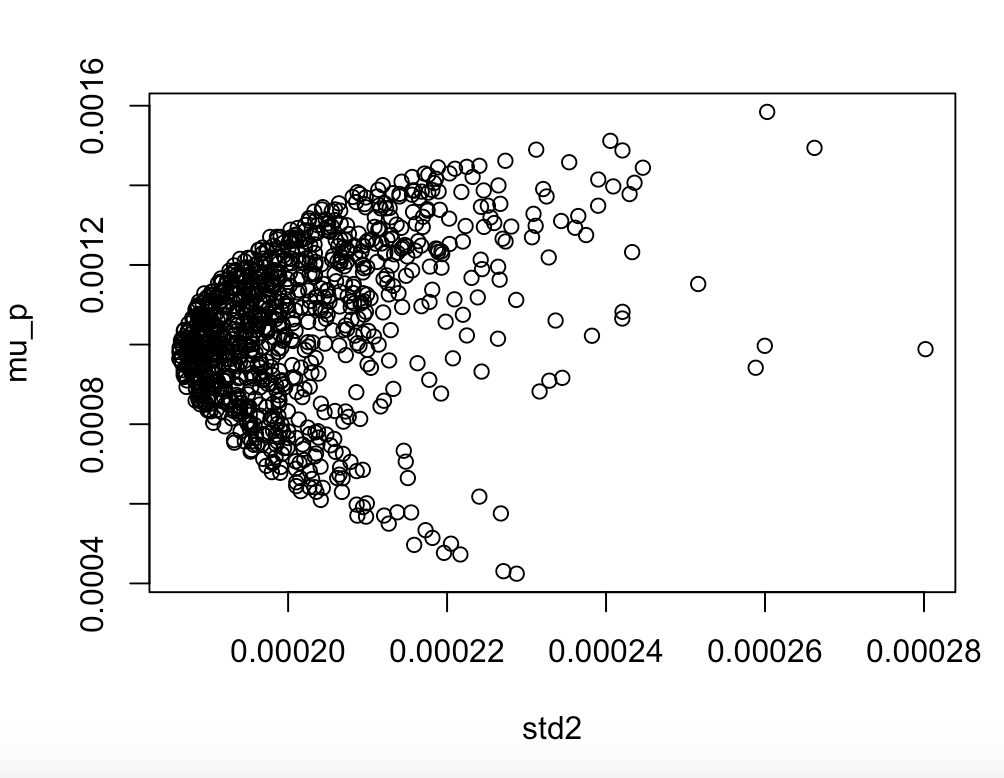
\includegraphics[width=0.7\linewidth]{ex1.png} 
    \caption*{Una muestra de la media y la varianza de 1000 portafolios aleatorios}
\end{figure}


\section*{Ejercicio 2}
Ahora nos centraremos en la frontera eficiente, un concepto importante en la optimización de carteras. La frontera eficiente representa un conjunto de carteras que ofrecen el rendimiento esperado máximo para un nivel dado de riesgo, o el riesgo mínimo para un nivel dado de rendimiento esperado. Al aprovechar los multiplicadores de Lagrange, buscamos derivar asignaciones de cartera óptimas.\\


El primer paso a realizar es construir el siguente vector:\\
%ponemos de r
% rbase <- seq(min(mitjanes),max(mitjanes),length=500)
Este es un vector de longitud 500 que va desde el valor mínimo de $\mu$ hasta su valor máximo dividiendo el intervalo en particiones iguales. \\

A continuación, crearemos el modelo lineal. Para ello, para cada elemento del vector que hemos creado, crearemos las matrices
\begin{equation*} Q =
\begin{pmatrix}
2C & \mu & \mathbb{1}\\
\mu^{t} & 0 & 0\\
\mathbb{1}^{t} & 0 & 0
\end{pmatrix}
\ b = \begin{pmatrix}
0\\
0\\
0\\
0\\
r \\
1
\end{pmatrix}
\end{equation*}
donde $\mathbb{1} = (1,1,1,1)^{t}$ y los valores C, $\mu$  son los que hemos definido en el apartado anterior. \\

Así pues, el código usado es \\

Sustituyendo los valores de C y $\mu$ conseguimos la siguente matriz:

\begin{equation*} Q =
\begin{pmatrix}
0.000694 & 0.000343 & 0.000237 & 0.000345 & 0.001718 & 1\\
0.000343 & 0.000525 & 0.000299 & 0.000273 & 0.001344 & 1\\
0.000237 & 0.000299 & 	
0.000568& 0.000313 & 0.000135 & 1 \\
0.000345 & 0.000273 & 0.000313 & 0.000634 & 0.001008 & 1\\
0.001718 &  0.001344 & 0.000135 & 0.001008 & 0 & 0 \\
1 & 1 & 1 & 1 & 0 & 0\\
\end{pmatrix}
\end{equation*}

Una vez tenemos estas marices definidas resolveremos el modelo lineal utilizando en R la funcion \texttt{solve}.

%poner codigos en r
%y<-solve(Q,b)

Obtenemos pues
\begin{equation*}
    y=
\begin{pmatrix}
-0.1012501\\
0.007596556\\
0.9205783\\
0.1730752 \\
0.2180101 \\
-0.0005847675
\end{pmatrix}
\end{equation*}
donde la solución es del tipo $$
\begin{pmatrix}
w_{r}\\
\lambda_{1}\\
\lambda{2}\\
\end{pmatrix}$$
Vemos que $w_{r}$ es un vector $1\times4$ que representa las ponderaciones de la cartera óptima con un nivel de rentabilidad determinado $r$
y $\lambda_{1}, \lambda{2}$ son los multiplicadores de Lagrange. \\

Por último, representaremos graficamente la frontera eficiente
\begin{center}
        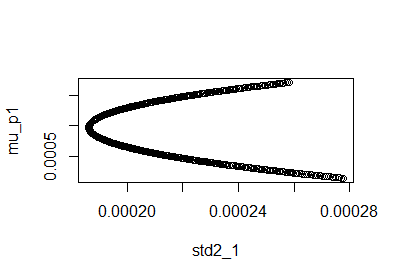
\includegraphics[scale=1]{Rplot11.png}
\end{center}

\section*{Ejercicio 3}
Para concluir, integraremos los resultados anteriores para presentar una representación visual de las posibilidades de inversión. Para ello vamos a trazar un gráfico que combina el conjunto factible de carteras, la frontera eficiente y la cartera de varianza mínima. \\

En el gráfico podemos observar las relaciones entre rendimiento y riesgo, éstas son fundamentales para la gestión de carteras. \\


\begin{center}
    \includegraphics[scale=0.7]{Gràfica.png}
\end{center}

Podemos ver que la línea negra trazada en el gráfico representa la frontera total de carteras. Los puntos azules dispersos a lo largo de la frontera total representan el conjunto factible de carteras. Estos puntos indican las combinaciones específicas de pesos en los activos que conforman carteras viables. La línea verde más gruesa destaca la frontera eficiente, que consiste en las carteras óptimas en términos de rendimiento para un nivel dado de riesgo. Finalmente el punto rojo en el gráfico indica la cartera de varianza mínima. Esta cartera representa la asignación de activos que minimiza la volatilidad o riesgo global.

\end{document}
